% ----------------- thesis chapters -----------
\chapter{Literature Review}
\label{chap: Literature}
This thesis is devoted to answering some of the key questions related to image recovery and dimensionality reduction in computer vision and pattern recognition applications. This thesis aims to address three key research goals: (1) construction of incoherent and robust sensing matrix for image compression using compressed sensing; (2) design of subspace learning algorithm for pattern recognition applications; and (3) design of regression-based feature extraction algorithm. In this chapter, we review some of the recent literature that are related to the above three research goals. 
%
\section{Sensing Matrix Optimization}
\label{sec: Chap2_Sensing_matrix}
%
The design of a sensing matrix to optimally select the informative samples from high-dimensional data is a challenging task. Several approaches have been proposed for this task, however conventional methods obtain the sensing matrix from the corresponding Gram matrix without considering the underlying structure of the equiangular frame. Tropp et al.~\cite{Frame} proposed a general alternating projection method that is capable of solving a large class of inverse eigenvalue problems which includes the construction of tight frames. For constructing a tight frame, they solve a matrix nearness problem based on the application requirements. In~\cite{Eva_frame}, the tight frames are constructed based on mutual coherence. The achieved mutual coherence is found to be close to the lower bound~\eqref{eq:welch} when the frame redundancy is not very high and can be employed for constructing frame of any dimension.
%\textcolor{red}{In this thesis, in addition to mutual coherence, we focus on restricting the eigenvalues of the Gram matrix in order to reduce restricted isometry constant, which in turn ensures tightness.} 
Next, Elad~\cite{Elad} initiated the work on sensing matrix optimization based on the averaged mutual coherence measure using a shrinkage scheme. Since mutual coherence considers worst-case correlation, it is not representative of the average reconstruction performance and the $t$-averaged mutual coherence is more appropriate. The authors in~\cite{Xuprojection} proposed a shrinkage function that projects the Gram matrix onto a non-empty convex set and reduces the off-diagonal elements towards the Welch bound. 

The authors in~\cite{Sapiro} proposed a method for designing the frame matrix by making a subset of its columns orthogonal, which is equivalent to minimizing the difference between the Gram matrix and the identity matrix (target ETF). A major advantage of this method is that it is non-iterative and offers significant computational improvement compared to~\cite{Elad}. Furthermore, Zelnik-Manor et al.~\cite{Zelnik} proposed an optimized sensing matrix design based on block-sparse representation which finds application in block-sparse decoding. Authors in~\cite{CHZ} focused on directly reducing the mutual coherence of the frame, and the optimized sensing matrix was designed by solving a non-smooth optimization problem with convergence guarantee. Similarly, Hong et al.~\cite{HONG_robust} optimized the sensing matrix based on the equivalent Gram matrix with a penalty term to minimize the sensing matrix energy. In~\cite{HONG_sparse}, an optimized sparse sensing matrix is constructed based on the target Gram matrix with a sensing matrix energy constraint. In~\cite{Vahid}, gradient-based alternating optimization approach is exploited to iteratively optimize the sensing matrix with decrements in the mutual coherence. Similarly, in~\cite{Measurement_Rahim}, the goal of optimization is to minimize the mutual coherence between the sensing and sparsifying matrix. An optimal sensing matrix is constructed based on the incoherent frame vectors, matrix nearness problem and initialization as a partial Fourier basis. Further, the work in~\cite{SRE_Huang} is focused on constructing an incoherent sensing matrix with an additional constraint on the sparse encoding error to ensure robustness. Bai et al.~\cite{SRE_Huang} optimize the sensing matrix such that the corresponding frame matrix approximates the target ETF. The method includes the sparse representation error to ensure robustness, however it employs the more sensitive Frobenius norm. Similarly, in~\cite{HONG_new_ref} and~\cite{Gangli_robust}, authors optimize the sensing matrix based on the Gram matrix using alternating optimization. Sparse representation error penalty is included to ensure robustness of the optimized projections. These methods focus on optimizing the sensing matrix based on the equivalent Gram matrix rather than using the ETF, which reduces the computational complexity and is physically more meaningful in order to achieve tightness among the frame vectors.
%
\section{Representation-based Feature Extraction}
\label{sec: Chap2_Sub_learn}
%
Feature extraction optimizes the projection basis to map the high-dimensional data to low-dimensional sub-spaces for dimensionality reduction while retaining the intrinsic structure of the data. Various approaches have been developed in this direction such as principal component analysis (PCA)~\cite{PCA}, linear discriminant analysis (LDA)~\cite{LDA}, neighbor preserving embedding (NPE)~\cite{NPE}, and locality preserving projections (LPPs)~\cite{LPP}. For dimensionality reduction, PCA solves the eigen decomposition problem and extracts the optimal vectors. LDA is a supervised method which exploits the label information to extract a discriminative and optimal projection matrix. LDA maximizes the between-class contrast and within-class similarity to obtain the optimal solution. However, PCA and LDA have some drawbacks. Both the approaches only consider the global structure of the data samples and neglect the local geometric structure. In addition, their performance degrades when the training samples are widely corrupted, e.g. varying expressions, poses, and illumination conditions. Also, LDA fails for the small sample size (SSS) problem i.e., the number of projections learned is limited by the scatter matrix. To alleviate these drawbacks, LDA based variants have been proposed, such as orthogonal LDA (OLDA)~\cite{OLDA} and manifold partition discriminant analysis (MPDA)~\cite{MPDA}. NPE and LPP utilizes the relationship between the data points and their neighbors to extract relevant features. The graph based projection learning methods~\cite{LPP,Sub_Adaptive_graph} can capture the intrinsic structure of the data. Many graph based methods pre-define the graph from the original data, which may suffer from the after-effects of random corruptions. Hence, adaptive graph learning is introduced to learn the relationship of data accurately~\cite{Sub_Adaptive_graph,Clustering_adaptive}.

Recently, representation-based methods have been proposed to address some of these limitations. Sparse representation-based classification (SRC)~\cite{SRC} exploits the sparse representation to constrain the representation matrix using the $\ell_{1}$-norm for classification. Motivated by SRC, collaborative representation-based classification (CRC)~\cite{CRC} uses the $\ell_{2}$-norm constraint instead of the $\ell_{1}$-norm, to encode the test data as a linear combination of the training data samples and reduce the computational cost. Locality-constrained linear coding (LLC)~\cite{LLC} utilizes the locality constraint with the representation coefficients by preserving the locality information while learning the coefficients. However, these methods do not exploit the relationship among the neighboring data samples. To address these drawbacks, low-rank representation (LRR) based methods~\cite{LRR_subspace,Learn_Bal_Unbal_graph} have been proposed based on the assumption that the intra-class samples lie on an intrinsic low-dimensional subspace. Thus, LRR can exploit the underlying structure of the data while addressing the impact of noise and outliers. Latent low-rank representation (LatLRR)~\cite{LatLRR} learns two low-rank projection matrices, one of which is used for feature extraction.

LRR-based methods have successfully extracted the low-rank global structure of the data; however, they are unable to provide dimensionality reduction-based feature extraction as they retain the dimensionality of the input data. In LatLRR, the number of the features learned is the same as the dimensionality of the original data. Recently, several approaches have been developed combining feature extraction and representation-based learning~\cite{PLR,LRE,RLSL,SRRS,SALPL,CDPL}. Low-rank embedding (LRE)~\cite{LRE} combines self-representation and projection learning into a single framework with a low-rank constraint on the coefficient matrix. LRE captures relationship between the data samples for reducing the impact of data corruption. Robust sparse LDA~\cite{RSLDA} uses the $\ell_{2,1}$-norm to extract more discriminative features. The algorithm optimizes the projection matrix with an orthogonal reconstruction matrix for improved performance.

In~\cite{RLSL}, a latent subspace is learned by jointly optimizing the subspace learning and the classification model parameters. However, it does not exploit the underlying global structure of the data. Similarly, supervised approximate low-rank projection learning (SALPL)~\cite{SALPL} learns a projection matrix by minimizing the classification error. In this line of work, latent low-rank and sparse embedding (LLRSE)~\cite{LLRSE} introduces $\ell_{2,1}$-norm regularization to extract and select the most discriminative features for the projection matrix. The robust $\ell_{2,1}$-norm enables LLRSE to be robust towards data corruption. However, these methods do not exploit the intra-class relationship among the data samples and do not perform well for the small sample size problems. Furthermore, the number of projections learned by SALPL and LLRSE is limited by the number of classes in the data set.
Constrained discriminative projection learning (CDPL)~\cite{CDPL} is a recently proposed approach that simultaneously searches for an optimal subspace for feature extraction and minimizes the classification error. CDPL exploits both the low-rank and sparse properties of the data for learning the projection. Nonetheless, CDPL has certain limitations which affect its classification performance. CDPL utilizes the precomputed Laplacian matrix of the binary graph to capture the consistency between the label information and the self-representation coefficients. The precomputed graph is derived from the original data, which may be corrupted with random pixel errors, occlusion, varying illumination conditions, and poses. The predefined graph does not preserve the nearest neighbor ranks as in the original data and hence cannot preserve the nearest neighbor structure of the data. CDPL does not explore the intrinsic structure of the transformed features and instead focuses only on learning the %similarity among the 
representation coefficients, which impairs the classification performance with small sample size.

Next, we briefly present the LRE~\cite{LRE}, SALPL~\cite{SALPL}, CDPL~\cite{CDPL} and LLRSE~\cite{LLRSE} methods for a better understanding of representation-based projection learning. These methods exploit the self-representation data to overcome the effects of data corruption. In these methods, sparse error constraint and regularizers are employed in unsupervised or supervised scenarios for learning optimal projections. 

Let $\bm{X} \in \Re^{m \times n}$ represent the original data matrix where $m$ is the dimensionality of the data and each column corresponds to a data sample. LRE exploits the self-representation property to learn projections as given below:
%
\begin{align}
    \begin{split}
        \label{eq: LRE}
        & \underset{\bm{P}, \bm{E},\bm{Z}}{\min} \quad \| \bm{E} \|_{2,1} + \lambda \| \bm{Z} \|_{*} \\
        & \hspace{0.3cm} \text{s.t.} \enskip \bm{P}^{T}\bm{X} = \bm{P}^{T}\bm{X}\bm{Z} + \bm{E}, \enskip \bm{P}^{T}\bm{P} =\bm{I}
    \end{split}
\end{align}
%
where $\bm{Z} \in \Re^{n \times n}$ represents the self-representation coefficients, $\bm{P} \in \Re^{m \times d}$ is the projection matrix with $d$ being the reduced dimension, and $\bm{E} \in \Re^{d \times n}$ is the error matrix. Here, $\|\bm{E}\|_{2,1}$ is the $\ell_{2,1}$-norm of $\bm{E}$ i.e., $\|\bm{E}\|_{2,1} = \sum_{i=1}^{d} \sqrt{\sum_{j=1}^{n} |\bm{E}_{i,j}|^{2}}$. LRE is one of the popular unsupervised subspace learning approaches capable of extracting significant features. 

Motivated by LRE, several supervised representation-based methods have been proposed. SALPL successfully integrates feature extraction and ridge regression as given below:
%
\begin{align}
    \begin{split}
        \label{eq: SALPL}
       & \underset{\bm{P}, \bm{Z}, \bm{R}, \bm{E}}{\min} \; \frac{1}{2} \| \bm{Y} - \bm{P}^{T}\bm{X} \|_{F}^{2} + \frac{\lambda_{1}}{2} \| \bm{P} \|_{F}^{2} + \lambda_{2} \| \bm{E} \|_{1} + \lambda_{3} \| \bm{Z} \|_{*} \\
        & \hspace{0.4cm} \text{s.t.} \hspace{0.5cm} \bm{X} = \bm{R}\bm{P}^{T} \bm{X} \bm{Z} + \bm{E}, \enskip \bm{R}^{T}\bm{R} = \bm{I}
    \end{split}
\end{align}
%
where $\bm{Y} \in \Re^{c \times n}$ is the binary label matrix and $\|\cdot\|_{F}$ represents the Frobenius norm. If $\bm{x}_i \in \Re^{m}$ belongs to the $j^\text{{th}}$ class, then the $j^{\text{th}}$ entry in the $i^{\text{th}}$ label vector $\bm{y}_{i} \in \Re^{c}$ is one and all other entries in $\bm{y}_{i}$ are zero.

Further, $\bm{P} \in \Re^{m \times c}$ works as a projection matrix with $d = c$, and $\bm{R} \in \Re^{m \times c}$ is included for data reconstruction. Here, the number of projections learnt is limited by the number of classes, and $\bm{R}^{T} \bm{R} = \bm{I}$ removes the orthogonal constraint on $\bm{P}$ for the ease of optimization. However, the optimized projections do not enable interpreting the significance of the features. To overcome this drawback, LLRSE employed the $\ell_{2,1}$-norm regularizer on the projection matrix $\bm{P}$ which encourages row sparsity. This allows LLRSE to extract more significant features while providing good interpretability for the importance of learnt features. 

CDPL integrates linear regression (LR) with subspace learning to learn optimal projections. To preserve the underlying geometric structure, CDPL employs the Laplacian regularizer on the representation coefficients as follows:
%
\begin{align}
  \begin{split}
     \label{eq: CDPL_form}
    & \underset{\bm{Z},\bm{E},\bm{W},\bm{D}}{\min} \, \| \bm{Z} \|_{*} + \lambda \|\bm{Z} \|_{1}  + \gamma \| \bm{E} \|_{2,1} + \beta \sum_{i,j} \| \bm{z}_{i} - \bm{z}_{j} \| \bm{B}_{i,j} + \frac{\alpha}{2} \| \bm{Y} - \bm{W} \bm{D} \|_{F}^{2} \\
         & \hspace{0.4cm}\text{s.t.} \hspace{0.5cm} \bm{P}^{T} \bm{X}  = \bm{P}^{T} \bm{X} \bm{Z} + \bm{E}, \enskip \bm{Z} \geq 0, \bm{P}^{T} \bm{P} = \bm{I}, \bm{Z} = \bm{J},  \enskip [\bm{P}^{T} \bm{X}; 1] = \bm{D}
    \end{split}
\end{align}
%
Here, $\bm{B}$ is the affinity or graph matrix precomputed from the original data space. CDPL utilizes both the low-rank and sparse structure characteristics for the representation coefficients. CDPL introduces a flexible transition matrix $\bm{W} \in \Re^{c \times d}$ from the low-dimensional subspace ($\bm{P}^{T} \bm{X}$) to the binary class label space ($\bm{Y}$). The flexibility of the transition enables CDPL to learn more number of projections than the class number $c$, and to handle the small sample size problem. However, as discussed earlier in this section, CDPL has certain limitations that impair its overall performance.
%
\section{Regression-based Feature Extraction}
\label{sec: Chap2_LSR}
%
Least square regression (LSR) is an efficient technique for classification by learning a mapping that can transform the data samples to the corresponding strict binary labels. In the last few decades, several regression analysis based methods have been proposed such as the ridge regression~\cite{Ridge_Regression,Kernel_ridge_PCA},
partial LSR~\cite{Partial_LS}, modified minimum squared error~\cite{Modified_MSE}, and least squares regularized regression~\cite{LS_RR}. In general, the conventional methods focus on employing the predefined binary label matrix as the regression target. However, it has been noted that the strict binary label matrix is not very appropriate for learning a discriminative transformation that can aid in the classification task~\cite{DLSR,ReLSR,GReLSR}. Discriminative LSR (DLSR)~\cite{DLSR} introduced the $\epsilon$-dragging technique which focuses on widening the margin between classes for regression. The primary objective of DLSR is to increase the inter-class margins by moving the regression targets of different classes along opposite directions by introducing a non-negative dragging matrix. Similarly, retargeted LSR (ReLSR)~\cite{ReLSR} can efficiently learn the regression targets from the training data while guaranteeing a large margin constraint for the classification of each data sample. Further, groupwise retargeted LSR (GReLSR)~\cite{GReLSR} %\textcolor{red}{proposed in 2018} 
exploits an additional regularization term to enhance intra-class similarity by explicitly defining and restricting the translation values in the ReLSR model. The objective of GReLSR is to introduce new flexible constraints to restrict regression target for multi-class classification. However, the resulting regression matrix does not allow interpretation of the significance of features i.e., the relative importance of the features with respect to one another. In~\cite{ICS_DLSR}, a sparse error term is introduced to relax the strict regression targets which in turn allows greater freedom in optimizing the projections. 

Next, we discuss the state-of-the-art algorithms for regression-based feature extraction. Let $\bm{X}=[\bm{x}_{1}, \bm{x}_{2}, \dots, \bm{x}_{n}] \in \Re^{m \times n}$ denote the data matrix with $\bm{Y} = \left[ \bm{y}_{1}, \bm{y}_{2}, \dots, \bm{y}_{n} \right]\in \Re^{c \times n}$ be the corresponding label matrix, where $c$ is the number of classes. In conventional LR, the label matrix $\bm{Y}$ is defined as a strict binary ($0/1$) matrix depending on the class information of the samples. Suppose $\bm{x}_{i} \in \Re^{m}$ belongs to the $j^{\text{th}}$ class, then the $j^{\text{th}}$ entry in the $i^{\text{th}}$ label vector $\bm{y}_{i} \in \Re^{c}$ is one and all other entries are zero. The LSR model can be formulated as:
% --------------------------------- %
\begin{equation}
    \label{eq: LSR}
    \min_{\bm{Q}} \, \|\bm{Q}^{T}\bm{X} - \bm{Y} \|_{F}^{2} + \lambda \| \bm{Q}\|_{F}^{2}
\end{equation}
%
where $\bm{Q}\in \Re^{m \times c}$ is the projection matrix and $\lambda$ is a regularization parameter. The LSR based algorithms proposed in recent years focus on employing the predefined binary label matrix $\bm{Y}$ as the regression target. Directly minimizing the regression loss between the projected (or transformed) features and binary labels is too restrictive and reduces the flexibility in learning the projection matrix. Furthermore, this does not allow the inter-class margins to be increased as the distance between the samples of two different classes in the label space is fixed at a constant value of $\sqrt{2}$. To address these limitations, various approaches have been proposed in the literature that allow learning more compact and discriminative regression targets. DLSR~\cite{DLSR} introduced the $\epsilon$-dragging technique which focuses on widening the margin between classes for regression. The objective function for DLSR is given as:
%  
\begin{equation}
    \label{eq: DLSR_obj}
     \min_{\bm{Q},\bm{M},\bm{b}}\, \| \bm{Q}^{T} \bm{X} + \bm{b} \bm{e}_{n}^{T}  - \bm{Y} - \bm{B}\odot \bm{M} \|_{F}^{2} + \lambda  \lVert\bm{Q}\rVert_{F}^{2}
\end{equation}
%
where $\bm{e}_{n} \in \Re^{n}$ is a vector with all $1$s, $\bm{b} \in \Re^{c}$ is an offset vector, $\odot$ represents Hadamard product, and $\bm{B} \in \Re^{c \times n}$ is given by:
%--------------------
\begin{equation}
    \bm{B}_{i,j} = \begin{cases}
    +1 \enskip \text{if} \enskip \bm{Y}_{i,j} = 1 \\
    -1 \enskip \text{if} \enskip \bm{Y}_{i,j} = 0
    \end{cases}
\end{equation}
%
The primary objective of DLSR is to increase the inter-class margins by moving the regression targets of different classes along opposite directions by introducing a non-negative dragging matrix $\bm{M}$. However, relaxing the strict label matrix using the $\epsilon$-dragging technique or with added margin also increases the distance between the regression responses of the intra-class samples thus potentially reducing the classification accuracy. This may also adversely affect the inherent local structure of the data. 

Retargeted LSR (ReLSR)~\cite{ReLSR} can efficiently learn the regression targets from the training data while guaranteeing a large margin constraint for the classification of each data sample. The ReLSR problem formulation is given by:
%
\begin{equation}
    \begin{split}
    \label{eq: ReLSR}
    \min_{\bm{Q},\bm{b},\bm{T}} \, \| & \bm{Q}^{T} \bm{X} +  \bm{b} \bm{e}_{n}^{T}  - \bm{T} \|_{F}^{2} + \lambda  \|\bm{Q}\|_{F}^{2}  \\
    \text{s.t.} \enskip & \bm{T}_{l_{i}, i} - \max_{j \neq i} \bm{T}_{j,i} \geq 1, \forall i = 1,2,\dots,n
    \end{split}
\end{equation}
%
where $n$ is the number of data samples in $\bm{X}$ and $l_{i} \in \{ 1,2,\dots, c\}$ is the class label corresponding to $\bm{x}_{i}$. However, ReLSR does not fully exploit the structural properties of the underlying data and only relies on the relaxed target matrix $\bm{T}$ for increasing the inter-class margins. 

GReLSR~\cite{GReLSR} employs an additional regularization term to enhance the intra-class similarity by explicitly defining and restricting the translation values in the ReLSR model. However, GReLSR does not exploit the robust $\ell_{2,1}$-norm for promoting row-sparsity in the projection matrix which would enable identifying the most discriminative features. In~\cite{ICS_DLSR}, a sparse error term is introduced to relax the strict regression targets which in turn allows greater freedom in optimizing the projections. Although~\cite{ICS_DLSR} exploits the row-sparsity property to ensure the transformed features of each class have a sparse structure, it does not consider the intra-class similarity among the data samples. In~\cite{RLSL}, Wang \emph{et al.} present the robust latent subspace learning (RLSL) which learns a transition subspace between the observed data and the binary labels, and provides a data representation that is more discriminative for classification. 
%
\section{Research Gaps}
\label{sec: Chap2_gaps}
%
From the preceding discussion on sensing matrix design algorithms (in Section~\ref{sec: Chap2_Sensing_matrix}), we list below the research gaps alongside highlighting some of the key frameworks in the literature for the design of ETF and optimization of the corresponding projection matrix. 
%
\begin{itemize}
%
\item The shrinkage scheme in~\cite{Elad} is computationally expensive and introduces a few large off-diagonal elements in the Gram matrix. Due to this, the worst-case guarantees for the recovery algorithms do not hold. The models discussed in~\cite{HONG_sparse, HONG_robust} result in only a slight reduction in the reconstruction error as the projection matrix is obtained directly from the designed Gram matrix. 
% Thus, we propose to optimize the frame matrix based on the target Gram matrix followed by optimization of the sensing matrix using the designed tight frame. 
\item The algorithms presented in~\cite{SRE_Huang, Gangli_robust} focus on optimizing the sensing matrix based on the equivalent Gram matrix rather than using the ETF. Moreover, these methods require the training data matrix as well as the sparse encoding error for the optimization of the sensing matrix, which is computationally expensive. 
%
\end{itemize} 
%
\noindent Next, we discuss some of the research gaps with respect to the feature extraction methods. Below we identify the limitations of the state-of-the-art algorithms discussed in Sections~\ref{sec: Chap2_Sub_learn} and~\ref{sec: Chap2_LSR}, and list the challenges addressed in this thesis.
%
\begin{itemize}
%
\item PCA~\cite{PCA} and LDA~\cite{LDA} consider the global structure of the data samples and neglect the local geometric structure. Due to this their performance degrades when the training samples are widely corrupted, e.g. varying expressions, poses, and illumination conditions. LDA~\cite{LDA} fails due to small sample size (SSS) i.e., as the number of projections learnt is limited by number of classes. 
%
\item SRC~\cite{SRC}, CRC~\cite{CRC}, LLC~\cite{LLC} methods are unable to exploit the inherent structure of the data samples. The low-rank representation~\cite{LRR_subspace, Learn_Bal_Unbal_graph, LatLRR} based methods have been successful in extracting the low-rank global structure of the data samples, however they do not come with the advantage of dimensionality reduction with feature extraction. In LatLRR~\cite{LatLRR}, the number of features learnt is same as the dimension of the original data space and hence does not result in dimensionality reduction.
%
\item The representation-based methods such as LRE~\cite{LRE}, SALPL~\cite{SALPL}, RLSL~\cite{RLSL}, LLRSE~\cite{LLRSE} do not exploit the intra-class similarity among the data samples and have poor classification accuracy for small sample size problems. Further, the number of projections learned by SALPL and LLRSE are limited by the number of classes in the data set. CDPL~\cite{CDPL} utilizes the pre-computed graph, which is unable to preserve the same nearest neighbor ranks as the original data and hence does not preserve the intrinsic nearest neighbor structure of the data. CDPL does not explore the underlying intrinsic structure of the transformed features, which leads to poor performance with small sample size. CDPL and LLRSE extract the optimal projections from the strict target matrix which is not the optimal discriminative target for correct classification.
%
\item In regression-based feature extraction approaches such as DLSR~\cite{DLSR}, relaxing the target matrix using the $\epsilon$-dragging technique increases the distance between the regression responses of the intra-class samples thus potentially reducing the classification accuracy. Retargeted LSR (ReLSR)~\cite{ReLSR} does not fully exploit the structural properties of the underlying data and only relies on the relaxed target matrix for increasing the inter-class margins. In GReLSR~\cite{GReLSR}, the resulting regression matrix does not interpret the significance of features, i.e., the relative importance of the features. The approach discussed in~\cite{ICS_DLSR} does not consider the intra-class similarity among the data samples.  
%
\end{itemize}
%
The research gaps discussed in two broad categories summarize the challenges that are addressed in this thesis. For CS-based system, the first research challenge is to design a sensing matrix with respect to the frame rather than the Gram matrix, which is physically more intuitive. Next, the designed sensing matrix needs to be incoherent and robust for real-world data for image reconstruction tasks. Similarly, for feature extraction methods, the challenges are to optimize low-dimensional features for data sets with wide intra-class variations, complex geometrical structures, and small training sample size.
%
\section{Motivation and Objectives}
\label{sec: Chap2_Mot_obj}
%
Following the research gaps identified in Section~\ref{sec: Chap2_gaps}, the motivation and objectives for this thesis are presented in this section. 
%The sensing matrix design and feature extraction are an active area of research for pattern recognition and computer vision applications. 
To address the research gaps, we present a brief summary of the objectives in two parts: (i) sensing matrix optimization and (ii) feature extraction. As discussed in Section~\ref{sec: chap1_hypothesis}, for CS-based sensing matrix optimization, the objective is to reconstruct original data from low-dimensional samples with a designed sensing matrix. For a well-designed CS-based image reconstruction model, the objectives are given below.\\ 
%
\noindent\textbf{Sensing matrix optimization}
%
\begin{itemize}
    \item To ensure reduced mutual coherence and improved tightness of the constructed equiangular tight frame.
    \item To incorporate sensing matrix energy constraint during the sensing matrix design for robustness.
    \item To adaptively minimize the sensing energy for improved robustness.
\end{itemize}
%
\noindent The next major objective is to extract significant and discriminative low-dimensional features for pattern recognition applications. In this context, some of the challenges are to preserve the underlying structure of the data, increase inter-class margins, and achieve good classification performance with small training sample size. Hence, the objectives for feature extraction (both representation and regression based) methods, are listed below.\\
%
\noindent\textbf{Feature extraction}
%
\begin{itemize}
    \item To achieve feature extraction and dimensionality reduction in a unified framework. 
    \item To improve the discriminative ability of the extracted features and to minimise overfitting. 
    \item To obtain larger number of projections than the number of classes and achieve improved classification performance.
    \item To capture the intrinsic structure of the data and adaptively preserve the neighborhood relationship among the data samples.
    \item For regression-based feature extraction, allow more freedom to the target matrix in optimizing projections to achieve enlarged inter-class margins.
    \item To capture the underlying structure of the data for improved classification performance.
    \item To maximize the intra-class similarity of the transformed features.
    \item To capture the underlying sparse structure for simultaneous extraction and selection of the most discriminative features. 
\end{itemize}

\section{Data Sets}
\label{sec: Chap2_Literature_datasets}
The following challenging benchmark data sets are used for the performance evaluation of the proposed sensing matrix design and feature extraction algorithms.\\
%
\textbf{Extended Yale B data set}: This data set is designed to evaluate the robustness of methods to the varying illumination influence~\cite{Yale_B}. It is composed of $2414$ frontal face images with poses from $38$ volunteers. Each class consists of $59-64$ images with different illuminations in each class, which makes face recognition quite challenging. 
%
\begin{figure}
\centering    
\subfigure[Ex Yale B data set]{\label{fig:Yale Dataset}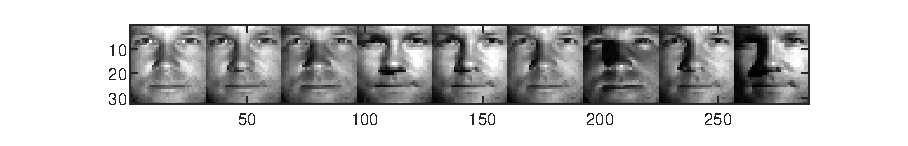
\includegraphics[keepaspectratio,width=0.80\textwidth,trim=17 0 40 2,clip]{fig_data/Yale_imagres.eps}}
\subfigure[AR data set]{\label{fig:AR Dataset}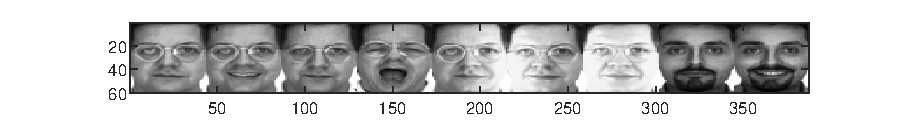
\includegraphics[keepaspectratio,width=0.80\textwidth,trim=17 0 40 2,clip]{fig_data/AR_images.eps}}
\subfigure[ORL data set]{\label{fig: ORL Dataset}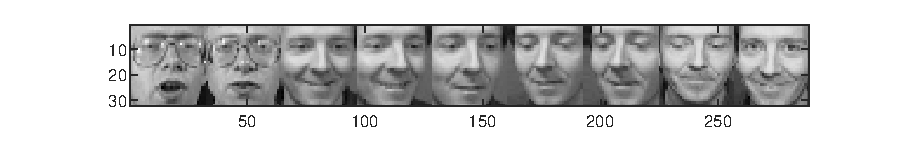
\includegraphics[keepaspectratio,width=0.80\textwidth,trim=17 10 40 2,clip]{fig_data/ORL_letter_images.eps}}
\subfigure[CMU PIE data set]{\label{fig:PIE Dataset}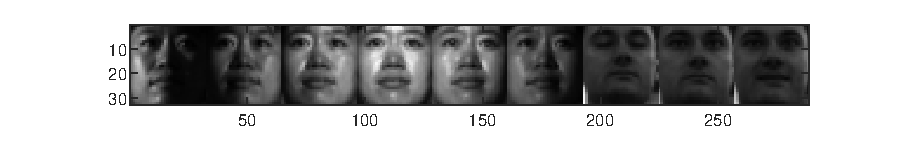
\includegraphics[keepaspectratio,width=0.80\textwidth,trim=10 10 40 2,clip]{fig_data/PIE_letter_images.eps}}
\caption{Sample images from the data sets used in this work for face recognition.}
\label{Fig: Sample Images_class}
\end{figure}
%
In all the experiments, each image is first resized to a dimensionality of $32 \times 32$ and then transformed into a vector. These vectors are stacked as columns to form a data matrix.\\
%
\noindent\textbf{AR data set}: In AR data set, there are $4000$ colour frontal face images from $126$ people ($56$ women and $70$ men)~\cite{Data_AR, LCKSVD}. Each volunteer provided $26$ images taken during two sessions. Each person provides $13$ images, in which $7$ images are with varying lighting, poses, and facial expressions, another $3$ with sunglasses, and the remaining $3$ with scarfs. Hence, the main challenges with the AR data set are the varying facial expressions, lighting conditions, and occlusions (such as sunglasses or scarfs). In this thesis, a subset containing $2600$ images from $50$ female and $50$ male subjects is used with the dimensionality reduced to $540$.\\
%
%
\begin{figure}
\centering    
\subfigure[Lena]{\label{fig:one}
\includegraphics[keepaspectratio,width=0.18\textwidth,trim=17 10 40 2,clip]{fig_data/lena.png}}
\subfigure[Barbara]{\label{fig:two}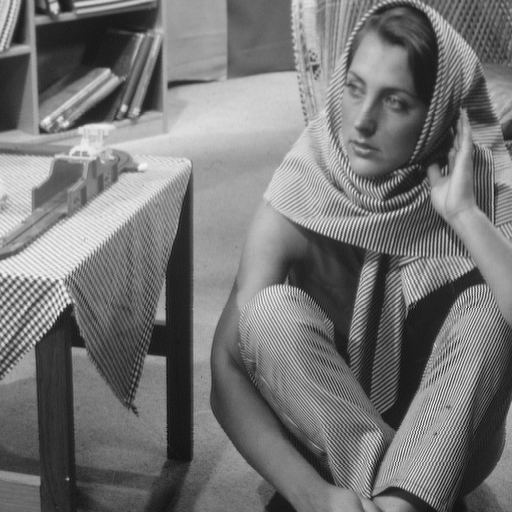
\includegraphics[keepaspectratio,width=0.18\textwidth,trim=17 10 40 2,clip]{fig_data/barbara.png}}
\subfigure[House]{\label{fig:four}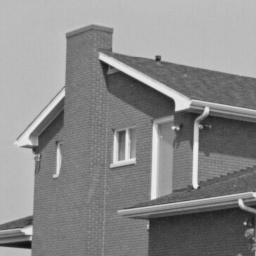
\includegraphics[keepaspectratio,width=0.16\textwidth,trim=10 2 40 2,clip]{fig_data/house.png}}
\subfigure[Cameraman]{\label{fig:five}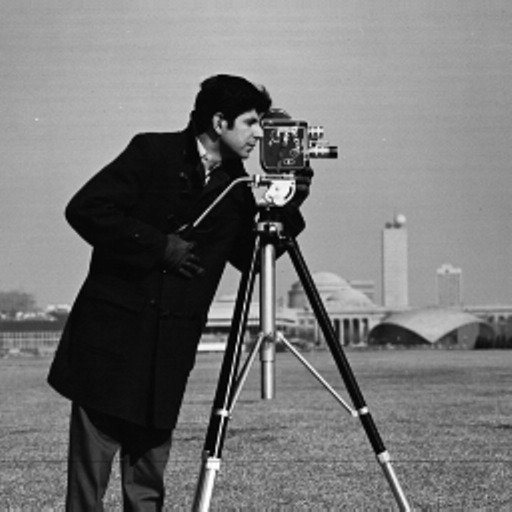
\includegraphics[keepaspectratio,width=0.18\textwidth,trim=10 0 40 2,clip]{fig_data/cam.png}}
\subfigure[Pirate]{\label{fig:seven}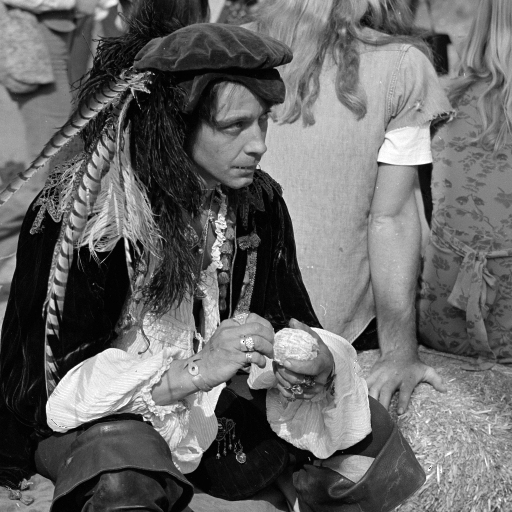
\includegraphics[keepaspectratio,width=0.18\textwidth,trim=10 0 40 2,clip]{fig_data/PirateTVinpainted.png}}
\caption{Some of the standard images used for image reconstruction.}
\label{Fig: Sample Images recog}
\end{figure}
%
\noindent\textbf{ORL data set}: The ORL face data set includes $400$ face images from $40$ persons with $10$ images per class (person)~\cite{ORL}. The main challenges with this data set are that the images were taken at different times, with varying lighting conditions, facial expressions, and facial details. We use cropped and resized images with a resolution of $32 \times 32$.\\
%
\noindent\textbf{CMU-PIE data set}: CMU-PIE data set is one of the challenging data sets for face classification as it consists of over $40,000$ images with various poses, lighting conditions, and facial expressions~\cite{CMU_PIE}. In this thesis, we use a subset of the CMU-PIE data set which contains $11,554$ images of $68$ subjects from the five frontal poses subsets $(\text{C}05, \text{C}07, \text{C}09, \text{C}27, \enskip \text{and} \enskip \text{C}29)$. Each image is resized to $32 \times 32$. There are nearly $170$ images with $5$ different poses in each class.
%
\begin{figure}
\centering  
\subfigure[COIL-20 data set]{\label{fig: COIL 20 Dataset}
\includegraphics[keepaspectratio,width=0.80\textwidth,trim=17 0 40 2,clip]{fig_data/COIL20.PNG}}
\subfigure[PubFig83 data set]{\label{fig:PFG Dataset}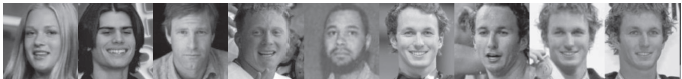
\includegraphics[keepaspectratio,width=0.80\textwidth,trim=17 0 40 2,clip]{fig_data/PFG.PNG}}
\subfigure[Caltech-101 data set]{\label{fig:Caltech Dataset}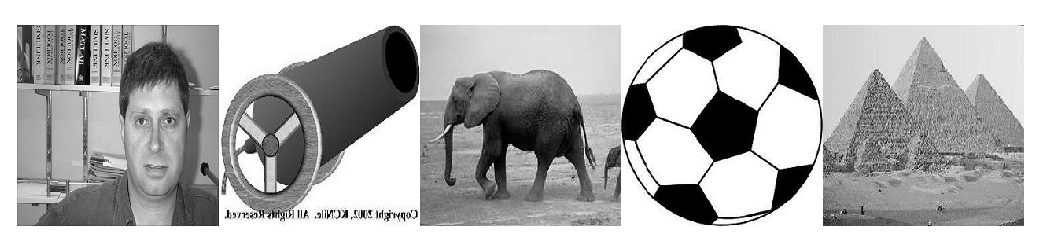
\includegraphics[keepaspectratio,width=0.80\textwidth,trim=10 10 40 2,clip]{fig_data/Caltech_images_letter.eps}}
\subfigure[15-Scene data set]{\label{fig: 15 Dataset}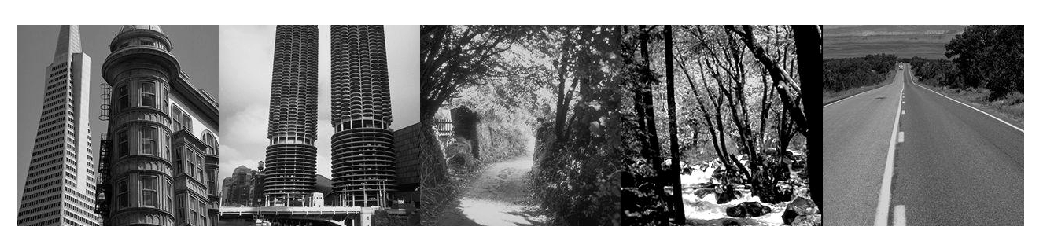
\includegraphics[keepaspectratio,width=0.80\textwidth,trim=0 10 40 2,clip]{fig_data/Scene_letter.eps}}
\caption{Sample images from the COIL-20, PubFig83, Caltech-101, and 15-Scene data sets used in this work for image classification.}
\label{Fig: Sample Images_class_2}
\end{figure}

\noindent\textbf{Caltech-101 data set}: In this thesis, we use the Caltech-101 data set to test our proposed methods for image reconstruction and object recognition~\cite{Caltech101}. The Caltech-101 is an extensively used data set for object recognition, which contains a total of $9146$ images with $101$ distinct object categories (faces, footballs, buildings, watches, pianos, and ants) and an additional background category. Each class has $31$–$800$ images with dimensionality roughly being $300 \times 200$.\\
%
\noindent\textbf{PubFig83 data set}: PubFig83 data set is a subset of the public PubFig data set~\cite{PubFig83}. PubFig83 consists of images collected from the web under unconstrained conditions~\cite{PubFig83}. In PubFig83 data set, each class contains more than $100$ samples with $83$ individuals and $13002$ face images. In this thesis, experiment is conducted on the feature set with dimensionality of $2048$ which comprises of histogram of oriented gradients (HOG), local binary pattern (LBP), and Gabor features extracted from the images.\\
%
\noindent\textbf{COIL-100 data set}: The COIL-100 image data set contains $100$ object images with each class comprised of $72$ gray-scale images~\cite{Data_COIL}. Similarly, COIL-20 data set consists of $20$ object images from each of the $72$ object classes. All the images are captured at pose interval of five degrees. The data set comprises of a wide variety of object images with complex geometric and reflectance characteristics such as toys, cups, vaseline jar etc. All the images were resized to $32 \times 32$ using the down-sampling algorithm. Further each image is transformed into a column vector of dimensionality $1024$ and stacked as columns of the data matrix.\\
%
\textbf{15-Scene data set}: 15-Scene categories data set is used for scene recognition. The data set is comprised of fifteen natural scene categories~\cite{15scene_1, 15scene_2, 15scene_3}. There are a total of $4485$ images for different categories such as bedrooms, kitchens, streets, stores, buildings, and country scenes. There are $200$ to $400$ images in each category. In this thesis, we used spatial pyramid features with a $4$-level spatial pyramid and a scale-invariant feature transform (SIFT) descriptor codebook with a size of $200$~\cite{LCKSVD}. Finally, dimensionality of the features is reduced to $3000$ using PCA. First, the SIFT descriptors are captured from $16 \times 16$ patches of the images computed over a grid with a step size of $8$ pixels~\cite{15scene_3}. Following the steps in~\cite{LCKSVD, 15scene_3}, we use the SIFT features for comparison with the state-of-the-art algorithms, and for higher discriminative power as dense features work better for scene classification.
